\documentclass{article}

%% preamble
\usepackage{hyperref}
\usepackage{verbatim}
\usepackage{color}
\usepackage{graphicx}
\usepackage{amsmath}

\topmargin 0pt
\advance \topmargin by -\headheight
\advance \topmargin by -\headsep
\textheight 9.in
\oddsidemargin 0pt
\evensidemargin \oddsidemargin
\marginparwidth 0.5in
\textwidth 6.5in
\newcommand{\myhrule}{ \begin{center}\rule{.9\linewidth}{.25mm}\end{center} }
\definecolor{darkgray}{rgb}{0.95,0.95,0.95}
\definecolor{heavygray}{rgb}{0.05,0.05,0.05}
\definecolor{foo}{rgb}{.8,0,.8}
\newcommand{\pad}{\vspace{8pt}\noindent}
\newcommand{\red}[1]{{\color{red}#1\color{black}}}
\newcommand{\myhref}[2]{\href{#1}{\color{foo}\underline{#2}\color{black}}}



\begin{document}

\title{CMDA 3634 Fall 2017 Homework 06}

%% change this to your name
\author{Kevin Jiang}
\vspace{-64pt}\maketitle
\begin{center}\underline{You must complete the following task by 11:59pm on 12/12/17.}\end{center}
Your write up for this homework should be presented in a {\LaTeX} formatted PDF document. You may copy the \LaTeX{} used to prepare this report as follows

\begin{enumerate}
\item Click on this  \myhref{https://www.sharelatex.com/read/vhrnbscgwfxk}{link} 
\item Click on Menu/Copy Project.
\item Modify the HW06.tex document to respond to the following questions. 
\item Remember: click the Recompile button to rebuild the document when you have made edits.
\item Remember: Change the author 
\end{enumerate}

\pad \emph{Each student} must individually upload the following files to the CMDA 3634 Canvas page at \myhref{https://canvas.vt.edu}{https://canvas.vt.edu}

\begin{enumerate}
\item \verb|firstnameLastnameHW06.tex| {\LaTeX} file.
\item Any figure files to be included by \verb|firstnameLastnameHW06.tex| file.
\item \verb|firstnameLastnameHW06.pdf| PDF file.
\item \verb|mcpi.r|, \verb|mcpi_mpi.r|, and \verb|mcpi_gpu.r| text file with student code. 
\end{enumerate}


\pad You must complete this assignment on your own. 

\vspace{16pt}
\begin{center}
\underline{\bf 100 points will be awarded for a successful completion.}
\vspace{8pt}\underline{\bf Extra credit will be awarded as appropriate.}
\end{center}

\newpage




\pad {\bf Q1} {\it (10 points) Serial Monte Carlo approximation of Pi.}
\vspace{8pt} 

\noindent 10 points will be awarded for submitting a serial Pi approximation method written in R. Submit code to canvas and push code to GitHub.

\myhrule

\pad {\bf Q2} {\it (20 points) Parallel Monte Carlo approximation of Pi.}
\vspace{8pt} 

\noindent 20 points will be awarded for submitting a parallel Pi approximation method written in R (using pbdMPI). Submit code to canvas and push code to GitHub.

\myhrule

\pad {\bf Q3} {\it (20 points) Strong Scaling Study of Parallel Pi Approximation Method.}
\vspace{8pt} 

\noindent For the strong scaling study, fix the total number of testpoint. Divide the total number of tests evenly among all processors. (You may have to alter your program slightly.) 
\begin{enumerate}
    \item Create a batch script that will build and run the code using 1, 2, 3, ..., 16 processors
    \item Submit your batch script on the newriver1 login node using qsub. 
    \item Plot a graph that shows how long it takes to run the Monte Carlo Pi approximation on the vertical y-axis, and number of processors used on the horizontal x-axis.
    \item Comment on your results. Does the code strong-scale perfectly ?
\end{enumerate}

\noindent Copy and paste the contents of the batch script file used to submit a job to newriver into your \LaTeX{} report. Include the plot mentioned above.  \\

Batch script:
\begin{verbatim}
    #PBS -ACMDA3634

    cd $PBS_O_WORKDIR
    
    #load R and R-parallel
    module purge
    module load intel mkl R/3.2.0
    module load openmpi hdf5 netcdf R-parallel/3.2.0
    
    #run the serial version
    #Rscript run_mcpi.r
    
    #run the parallel version with parRapply
    #Rscript mcpi_parallel_apply.r
    
    #run the parallel version with mclapply
    #Rscript mcpi_parallel_mc.r
    
    #run the pbdr version
    for i in {1..16}
    do
    mpiexec -np $i Rscript mcpi_pbdr.r
    done
\end{verbatim}

\begin{figure}[ht!]
    \centering
    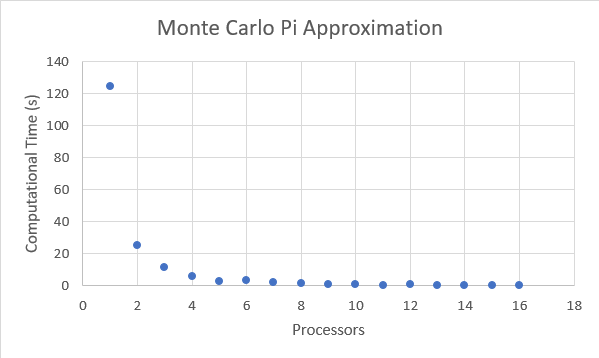
\includegraphics{monte_carlo_pi_times.png}
    \caption{Monte Carlo Pi strong scaling}
    \label{fig:monte_carlo_graph}
\end{figure}

Based on the graph produced, the code does strong-scale perfectly although the times are not as consistent despite increasing the number of processors.  However, overall, the model fairly produces an accurate trend line.

\myhrule

\pad {\bf Q4} {\it (20 points) Weak Scaling Study of Parallel Pi Approximation Method.}
\vspace{8pt} 

\noindent For the weak scaling study, have each processor run on do the same amount of work. That is, the total number of points tested should increase linearly with number of processors run on. (You may have to alter your program slightly.)
\begin{enumerate}
    \item Create a batch script that will build and run the code using 1, 2, 3, ..., 16 processors
    \item Submit your batch script on the newriver1 login node using qsub. 
    \item Plot a graph that shows how long it takes to run the Monte Carlo Pi approximation on the vertical y-axis, and number of processors times testpoints per node used on the horizontal x-axis.
    \item Comment on your results. Does the code weak-scale perfectly ?
\end{enumerate}

\noindent Copy and paste the contents of the batch script file used to submit a job to newriver into your \LaTeX{} report. Include the plot mentioned above.  \\

Batch script:
\begin{verbatim}
    #PBS -ACMDA3634

    cd $PBS_O_WORKDIR
    
    #load R and R-parallel
    module purge
    module load intel mkl R/3.2.0
    module load openmpi hdf5 netcdf R-parallel/3.2.0
    
    #run the serial version
    #Rscript run_mcpi.r
    
    #run the parallel version with parRapply
    #Rscript mcpi_parallel_apply.r
    
    #run the parallel version with mclapply
    #Rscript mcpi_parallel_mc.r
    
    #run the pbdr version
    for i in {1..16}
    do
    mpiexec -np $i Rscript mcpi_pbdr.r
    done
\end{verbatim}

\begin{figure}[!ht]
    \centering
    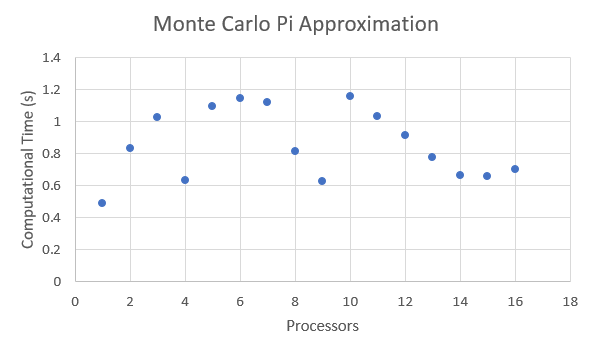
\includegraphics{monte_carlo_pi_weak.png}
    \caption{Monte Carlo Pi weak scaling}
    \label{fig:my_label}
\end{figure}

NOTE: I reduced the points size from 1e7 to 1e5 in the interest of time. \\

Based on the graph produced, the code does weak-scale, although it seems a bit sporadic.  
\myhrule

\pad {\bf Q5} {\it (30 points) GPU-R Monte Carlo approximation of Pi.}
\vspace{8pt} 

\noindent Use GPU-R to create a Monte Carlo approximation of Pi. Document the time it takes to run the program. How does it compare to the serial program? How does it compare to the parallel R program run on various numbers of processors? \\

\noindent Submit code to canvas and push code to GitHub. \\

I was unable to figure this question since I am still unfamiliar with R's syntax.

\myhrule

\pad {\bf Extra Credit:} {\it (50 points) Vectorized Monte Carlo Estimation of Pi with Scaling Study .}
\vspace{8pt} 

\noindent Vectorize the mcpi.r program for a further speed up. (Hint: Some default R functions, for instance \texttt{apply}, use for loops under the hood.) If the program is vectorized correctly, expect a speed up factor of about 50. \\


\noindent Once the program is vectorized, repeat the scaling studies performed in \textbf{Q3} and \textbf{Q4} with the vectorized code. In addition to plotting the results on there own plots, graph the results from the strong scaling study of the non-vectorized and vectorized programs on a single plot. (You might consider taking the log of the y-axis for this plot. Label axis clearly.) Comment on your results. Compare and contrast the scaling of the vectorized and non-vectorized codes.




%%\begin{thebibliography}{9}

%%\end{thebibliography}


\end{document}